\title{Aggressive Scheduling for Numerical Programs}
\author{Richard Veras, Flavio Cruz, Berkin Akin}
\date{\today}
\documentclass[10pt]{article}

\usepackage{url}
\usepackage{verbatim}
\usepackage{amsmath}
\usepackage{amsfonts}   % if you want the fonts
\usepackage{amssymb}    % if you want extra symbols
\usepackage{listings}
%\usepackage{savetrees}
\usepackage{graphicx}

\begin{document}

\maketitle

\begin{abstract}
   Certain classes of algorithms are still hard to optimize by modern compilers
   due to the differences between computer architectures.
   Numerical algorithms, for example, perform better when taking advantage of features
   such as software pipelining and loop unrolling. Expert programmers are usually able to
   get the last drop of performance from the hardware, however, compilers cannot perform the same
   feat for loss of generality. The SPIRAL system bridges this gap by generating machine specific code
   from high level algorithmic descriptions. We used the SPIRAL system to implement software
   pipelining for numerical algorithms with XXX (talk about scheduling). Our results show that
   by unrolling and applying software pipelining at the C code level, we can
   improve performance by up to 30\% over unrolling alone.
\end{abstract}

\section{Introduction}

Modern compilers are able to transform relatively slow code into fast code
by performing several optimizations. The majority of such optimizations
are geared towards general purpose code that is typically full of memory operations and
branches. This makes sense, since the code that most programmers write falls into this category.

However, there are certain classes of algorithms where this approach falls short in improving
the performance of the target code. One good example is numerical code. Expert programmers
are able to take a very na\"\i ve implementation and then fine tune it to take advantage of the
micro-architecture features of the target machine. Such features include things like software
pipelining~\cite{Rau:81} (for improving the performance of Out-Of-Order execution by interleaving loop iterations),
unrolling (by knowing how big are the memory caches of the processor) and pre-fetching.
Unfortunately, compilers are unable to perform such optimizations due
to some loss of generality and also because most optimizations performed by a compiler
cannot see the forest for the trees, and thus can't take into account a complete numerical algorithm.
This problem is further emphasized by the fact that expert programmers test and tune various permutations
of their code and its scheduling of instructions, a task that compilers are usually unable to do because
they would have to guess the structure of the input data and then generate and run small instances of the problem
to find an optimal solution.

Automatic Program Generation Systems like SPIRAL~\cite{Pueschel:05} are tools that produce a system
dependent and highly optimized implementation of an operation from a very high level mathematical description. 
This is achieved though three mechanisms: a language that captures the algorithmic details of an operation, a powerful
rewriting mechanism that uses that knowledge to map these algorithms to the special features of the hardware (vector
instructions and parallelism), and a backend code generator that produces a tuned implementation in a high-level language
(usually C). The later component provides a means for SPIRAL to be portable by allowing modern compilers to do the task
of transforming C code to assembly.

However, because SPIRAL uses C as the target language, this comes at a cost since there is no control over register allocation and
scheduling. Scheduling in particular plays a very important role in the performance of numerical code. Even on an Out-of-Order
processor long dependency chains can drastically degrade performance. Thus, the goal of our project is to incorporate scheduling,
namely Software Pipelining, into SPIRAL in a way that we can produce highly-tuned schedules for target architectures.
This way, we can still use the optimizations available in modern compilers while also performing aggressive scheduling optimizations
that only experts would be able to do.

In this project we explore the problem of scheduling code at the high-level and generate high-performance code that is comparable
to an expert. XXX

\begin{comment}
+( ) APGS aim to replace expert programmers for high-performance code.
+( ) For some classes of operations they have been very successful, but for
  others they fall short in performance.

+( ) Most expert programmers code their implementations in low-level assembly
  code and perform micro-architectural specific optimizations that production
  compilers cannot do for loss of generality.

+( ) This is further aggravated by the fact that experts test and tune various
  permutations of their code and its scheduling, a task that compilers do not
  do for the same reasoning as above.

+( ) Even on out-of-order machines scheduling at the code level is important
     to minimize the effects of long dependency chains that can cause the
     system to behave like an in-order processor.


+( ) APGS tune and optimize an implementation of an operations from the
  algorithmic level down to the low level just as an expert would, but because
  these systems rely on a high-level language like C as a target instead of
  assembly.

+( ) As a result these systems must rely on the compiler for instruction
  scheduling.

+( ) One could target assembly instead of a higher-level language but that
  defeats the purpose of having a portable system that can generate
  specialized code

+( ) How can we effectively schedule code at the high-level and generate
  high-performance code that is comparable to an expert.
\end{comment}

\subsection{Our Approach}

To approach this problem, we are directly using SPIRAL \emph{intermediate code} (called ICode)
to represent several numerical algorithms. Any optimization performed at this level can benefit
lower level code.

We apply several optimizations to the ICode representation of our algorithms. For example,
for loop unrolling and loop tilling (or loop blocking), we have several parameters that allows
us to set how much unrolling will be done in the inner loop and the size of the tile.
This gives us great freedom to select the best parameters that will make our final code more
performant. In addition to these, we also apply software pipelining to the original code.
We create three states, namely prologue, steady state, and epilogue, to setup, run and finish
the pipelined computation, respectively.

After these transformations, we generate C code from ICode. Of course, the final code will
have all the optimizations performed at the ICode level, however we have developed a technique that
forces the target C compiler to obey the scheduling we have set up during the software pipelining
transformation. Usually, C compilers tend to remove such scheduling and perform their own optimizations,
which is not what we want.

Our approach gives us several advantages. The first one is that we are able to generate fully optimized
code using software pipelining from a high level description. The second and final advantage, is that
we are still able to use the nice features provided by the C compiler (specially portability)
while tuning the scheduling parameters. 


\begin{comment}
+( ) Work directly in the SPIRAL intermediate code. Any optimization that is done
  here can benefit any operation expressed at a higher level of abstraction.

+( ) We use Software Pipelining in addition to loop unrolling and other
  optimizations that we can fine tune.

+( ) We generate the target code in C and use a quality production compiler.

+( ) But we instrument our code in such a way that we can force a particular
  schedule on our code.

+( ) Thus we get all of the benefits of APGS and the ability to even tune
  schedules, but we can still take advantage of the compiler for dealing with
  mapping our implementation to assembly (reg alloc and such).
\end{comment}

\subsection{Related Work}

Much research has been done to automatically generate the best implementation
for a given architecture using tunable parameters. These parameters are
related to standard techniques such as loop transformations, loop tilling and loop unrolling.
In these research systems, there is a procedure that searches for the best combination of optimizations
that will generate the most performant implementation.

A very well-known system is ATLAS \cite{Whaley00automatedempirical} (Automatically Tuned Linear Algebra Software).
It automatically generates high performant numerical libraries known as the BLAS~\cite{Lawson:79} (Basic Linear Algebra Subprograms)
using \emph{global search} over the optimization parameters. Many programs are generated with different combinations
and then run on the actual hardware to determine the best values that give the best performance.
ATLAS can also make use of hand-coded BLAS routines in the case that the best solution performs worse than the hand-coded version.

FFTW3~\cite{Frigo05thedesign} is also similar to ATLAS, although FFTW3 targets the implementation of the Discrete Fourier Transform.
FFTW3 uses the concept of a \emph{planner} that receives as input the shape of the input data (array sizes, memory layouts, etc).
The planner returns a \emph{plan} that is able to solve the problem using data that conforms to the initial shape. The planner measures
the execution time of different plans and selects the best one. FFTW3 results show that the best plan performs very close
to what an expert would do.

While both ATLAS and FFTW3 use the same global search principle, Yotov~\cite{Yotov05issearch} showed that it is possible to get
similar results just by using traditional \emph{analytical models}. In his work, he modified the search engine of ATLAS to use
a model parameter estimator that receives hardware information (L1 cache size, number of registers, etc) and outputs
one implementation of the target algorithm that should be best suited for the input parameters. Yotov wanted to show that
traditional compilers should be able to get similar results as ATLAS without the need to execute multiple versions of the same
algorithm to find the best solution. He showed that model driven optimization can achieve very similar results, without the need
to do extensive and time consuming empirical search.

\begin{comment}
+( ) OSKI
+( ) FFTW
+( ) ATLAS/PhiPack
+( ) [Yotov] discusses how ATLAS only needed fine tuning and many of the course
  adjustments could be determined analytically.
+( ) Lam's software pipelining technique
\end{comment}

Software pipelining was a technique invented by Patel and Davidson~\cite{Patel:76} for scheduling hardware pipelines.
Later, Rau and Glaeser~\cite{Rau:81} were able to implement software pipelining in a compiler. In her seminal paper,
Lam~\cite{Lam:88} showed that it is possible to implement
software pipelining without hardware support and just instruction-level parallelism. This can be accomplished by using modulo variable
expansion and unrolling of the loop code a small number of times, a technique called \emph{modulo renaming}.
Lam also noted that inter-iteration dependences in a loop can create cycles in the dependence graph and therefore constraint the
scheduling of all other instructions. Lam presented some techniques to deal with this problem.

\subsection{Our Contributions}

The contributions of this paper are the following:

\begin{description}
   \item[Software Pipelining] We developed a transform that takes a numerical algorithm and adds software pipelining support
   using three stages. We are able to use this optimization along with other optimizations such as loop unrolling and loop tilling.
   Moreover, we were able to apply a technique that disallows C compilers to perform their own scheduling to the code. At the same
   time, we still use all the other optimizations provided by the C compiler. 
   \item[Evaluation] We evaluated our programs using several tunable parameters for software pipelining,
   loop unrolling and loop tilling. The results XXX
\end{description}

\begin{comment}
+( ) A general technique(hack) for forcing schedules in C
+( ) An implemented set of rules in SPIRAL for tunable software pipelining.
+( ) And as a result, potentially faster code that is generated by SPIRAL that is
  comparable to an expert.
\end{comment}

\begin{comment}
   Given a loop described at the ICode level we want to do three things:
   0. Apply a transformation to turn it into a 3 software pipelined loops
   (prologue, steady state, and epilogue). The prologue and the epilogue
   space out computation as best as possible while preserving ordering. And
   the steady state mirrors the original loop in terms of the order of
   instructions, but the elements that each instruction is operating on are
   from different loop iterations.

   1. We want unroll all 3 of the loops. We do this because we don't want
   to deal with register allocation (this would involve implementing
   iterative-modulo scheduling), we would rather let the compiler figure
   out the allocations instead. As a bonus, we drop the loop overhead.

   2. Then we want to instrument those instructions with labels from goto
   statements, so we can force the schedule. By placing a label between
   each instruction and making the control flow unpredictable at compile
   time, the compiler is forced to preserve this schedule.
\end{comment}


\section{Details Regarding Design}

% I feel this repeats the introduction
SPIRAL is an Automatic Program Generation System (APGS) that exploits the mathematical
structure of algorithms to optimize and fine tune them. Most compilers do
a poor job of compiling mathematical/numerical algorithms since they don't take advantage
of the underlying computer architecture. SPIRAL is a feedback-driven compiler because
it explores the capabilities of the target machine and tries to find the best
implementation, comparable to the one that would be hand-written by an expert programmer.
SPIRAL is thus the perfect tool to exploit software pipelining in numeral algorithms.

SPIRAL code is used to declare high level mathematical operations which compiled gets transformed
into ICode. ICode is the intermediate representation that SPIRAL uses before the code is compiled into C code.
It represents the abstract syntax tree (AST) of the parsed program.
It is also possible to write programs in ICode. An example of ICode is presented in Fig.~\ref{fig:dswap}.
It declares a function that receives two vectors (\texttt{x} and \texttt{y}) and swaps their values.
In the example, we use unrolling (the second \texttt{loop} construct) to optimize the performance.
This program has three parameters: \texttt{datatype}, to select the datatype of the vectors;
\texttt{loop\_bound}, to select the size of both vectors; and, \texttt{unroll\_bound} to select the unrolling factor.

\lstset{basicstyle=\tiny}

\begin{figure}[ht]
\begin{lstlisting}
swap := (datatype,
            loop_bound,
            unroll_bound) -> let(

   x := var("x", TPtr(datatype)),
   y := var("y", TPtr(datatype)),
   it := var("i", TInt),
   it2 := var("ii", TInt),
   actuali := var("act", TArray(TInt, loop_bound)),
   temp := var("temp", TArray(datatype, loop_bound)),

   program(
      chain(
         func(TVoid, "swap", [x, y],
            decl(Concatenation([it],
                  getVarArrayNames("temp", unroll_bound, datatype),
                  getVarArrayNames("act", unroll_bound, TInt)),
               chain(
                  loop(it, loop_bound/unroll_bound,
                     FlattenCode(loop(it2, unroll_bound,
                        chain(
                           assign(nthVar(actuali, it2), add(it2, mul(it, unroll_bound))),
                           assign(nthVar(temp, it2), nth(x, nthVar(actuali, it2))),
                           assign(nth(x, nthVar(actuali, it2)), nth(y, nthVar(actuali, it2))),
                           assign(nth(y, nthVar(actuali, it2)), nthVar(temp, it2))
                     )).unroll())
                  )
               )
            )
         )
   )
));
\end{lstlisting}
\caption{Swap Example}
\label{fig:dswap}
\end{figure}

We can ultimately compile the example in Fig.~\ref{fig:dswap} to C code. If we compile the call to \texttt{swap(TInt, 20, 2)}
we get the C code in Fig.~\ref{fig:dswap_compiled}.

\lstset{basicstyle=\small,language=C}

\begin{figure}[ht]
\begin{lstlisting}
void swap(int  *x, int  *y) {
    int act_0, act_1, i, temp_0, temp_1;
    for(i = 0; i <= 9; i++) {
        act_0 = (i*2);
        temp_0 = x[act_0];
        x[act_0] = y[act_0];
        y[act_0] = temp_0;
        act_1 = (1 + (i*2));
        temp_1 = x[act_1];
        x[act_1] = y[act_1];
        y[act_1] = temp_1;
    }
}
\end{lstlisting}
\label{fig:dswap_compiled}
\end{figure}

\subsection{Software Pipelining}

Software pipelining is a coding technique that optimizes loops by overlapping instructions
from different loop iterations in order to exploit instruction level parallelism.
Due to this overlap we say that software pipelining is a type of out-of-order execution.
While software pipelining is somewhat similar to hardware pipelining, the order of the executions
is not determined by the processor but by the compiler or the programmer.

With software pipelining, we can reduce
pipeline stalls in the hardware, since the pipeline can be fed with new instructions from
different loop iterations. This greatly increases instruction parallelism because we can
start a new loop iteration before the past ones have completed. For this technique to be
effective, the loop is transformed into three sections:

\begin{description}
   \item[Prologue:] We start adding several iterations to the hardware pipeline.
   This phase ends when the last instruction of the first instruction is to be executed.

   \item[Steady State:] This phase starts where the prologue ends. Most execution time is spent
   here and this finishes when the first instruction of the last iteration is executed.

   \item[Epilogue:] In this phase, the hardware pipeline executes the last remaining instructions.
\end{description}

The need to duplicate the loop code into three phases is a notorious disadvantage of software
pipelining, because it may increase the program's code size. Moreover, since software pipelining
is usually used in conjunction with loop unrolling, this enlarges the code
even more. While this can be an issue on processors with little to no
instruction cache, in practice on most modern systems this is not an issue.

The implementation of software pipelining in SPIRAL was straightforward, and
involved three indexing functions each for the prologue, epilogue and steady
state, which mapped the instructions in a fully unrolled loop to its correct
position in an unrolled and software pipelined loop.

Additionally, by targeting unrolled code we were able to bypass the need to do
register allocation in SPIRAL. By insuring that the number of instructions in the
pipelined loop is less than the number of registers on the system, the
compiler was able to allocate registers with little to no spills.


\subsection{Enforcing a Schedule}
\begin{comment}
+(X) How do we enforce a schedule at the C level?
+( ) What does the code look like?
+(X) Would this hack always work? Either way it would be ideal to have a flag
     or pragma to allow the user to choose a schedule.

\end{comment}

Most modern compilers do not preserve instruction ordering imposed at the
input language level, and instead rely on general purpose methods such
as \emph{list scheduling} to order instructions. In the common case, this frees
the developer from the task of determining an efficient schedule, but in our
case this feature serves as a roadblock. While the GCC~\cite{gccwebsite} provides flags for
disabling instruction scheduling it comes at the cost of overall
performance because we only plan to schedule loop code. Moreover, our plan
involves using the Intel Compiler~\cite{iccwebsite}, thus we need a general solution for
scheduling at the C code level.

In order to enforce a schedule at the C code level we need to prevent the
compiler from imposing its own scheduling. A compiler must preserve the
semantics of the input code, so to take advantage of this fact we place a
label before each instruction with a \emph{goto} nested in
a \emph{switch-case} block. We declare the value for the \emph{switch}
statement as a global variable set such that the code will always jump to the
first instruction. Initially, we simply embedded each instruction in
a \emph{switch-case} block, but both the GCC and Intel compiler would create
multiple code paths and schedule each path individually. Fig.~\ref{fig:force_sched} shows
an example of our method in practice.

For our purposes this technique proved itself effective for enforcing a
schedule, but in some cases the GCC compiler would add superfluous instructions. Thus
in the future a more general approach, such as a compiler directive, would be
advantageous.


\begin{figure}[ht]
\begin{lstlisting}
int state=0;

void test(double  *Y, double  *X) {
    switch(state) {
      case 1: {
      goto label1;        }
      case 2: {
      goto label2;        }
      /* .... snip .... */
      case 26: {
      goto label26;        }
      case 27: {
      goto label27;        }
    }

    label1:
    a91 = (X + 1);
    label2:
    a95 = *(X);
    /* .... snip .... */
    label26:
    a111 = *(a94);
    label27:
    a112 = (Y + 3);
}


\end{lstlisting}
\caption{A template for enforcing an instruction ordering in C.}
\label{fig:force_sched}
\end{figure}


\subsection{Putting it all Together}
\begin{verbatim}
+( ) Requirements of the code before we can SP (what optimizations should we
  do/evaluate automatically?)

\end{verbatim}

\section{Experimental Setup}
\begin{verbatim}
+( ) What do we want to demonstrate? Software pipelining can improve the
     performance even on Out-of-order machines.

+( ) What machines will benefit the most from this?

+( ) What operations will benefit the most?

+( ) We want to show the breakdown of the cycles for each test and where the
     stalls were occurring.
+( ) What is our testbed? What machines do we use?
\end{verbatim}


\section{Experimental Evaluation}

\begin{verbatim}
+ What algorithms are we using?
+ What systems are we using?

+ What does the SimpleScalare results show? What systems benefit the most?
Which ones benefit the least?

+ How can we fine tune the SP parameters to a system? This is where we vary
the delays. For example the first few instruction of a loop will most likely
be loads and the rest will be computations, so can we cluster the memory ops
and issue them well before the computations.

\end{verbatim}


%% I know this is ugly, but if you have the chance Flavio can you beautify
%% this with side-by-side figures
\begin{figure}[ht]
\begin{center}
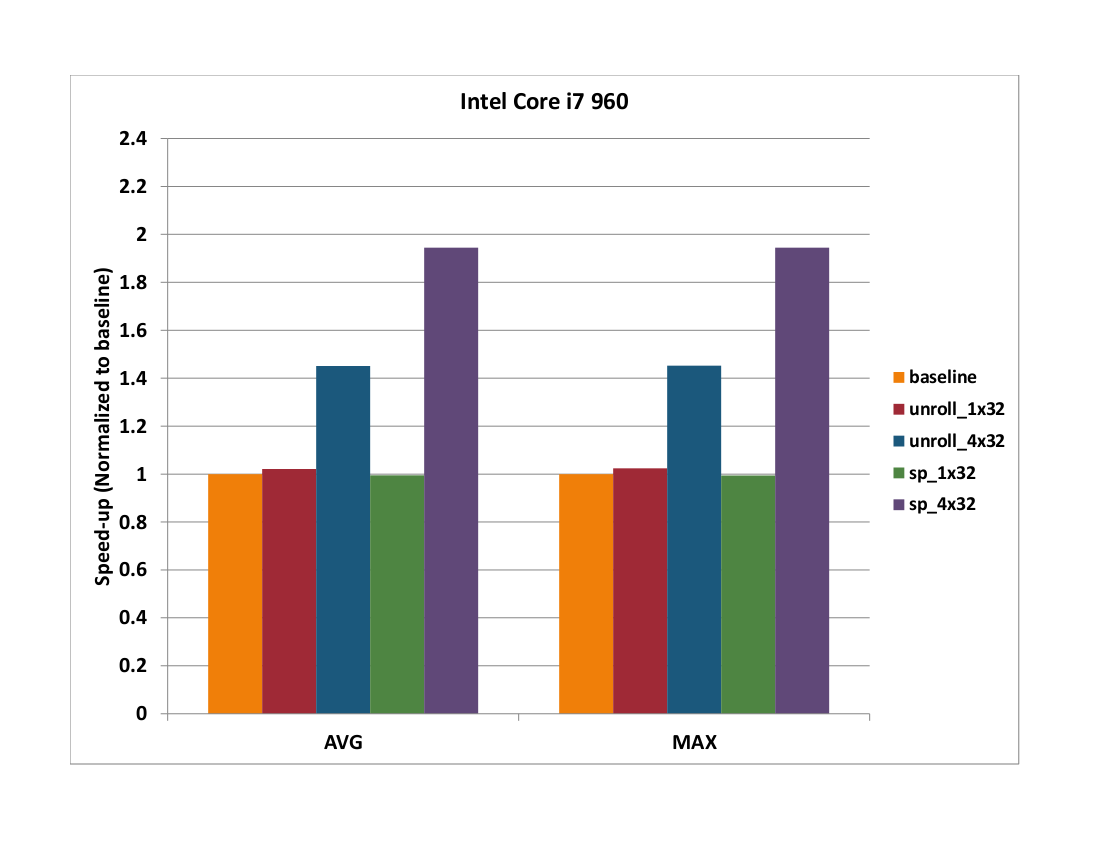
\includegraphics[scale=.5]{gemv_intel_core_i7_960.png}
\end{center}
\caption{Relative speedup of GEMV on the Intel Core i7 960.}
\label{fig:gemv_corei7}
\end{figure}

\begin{figure}[ht]
\begin{center}
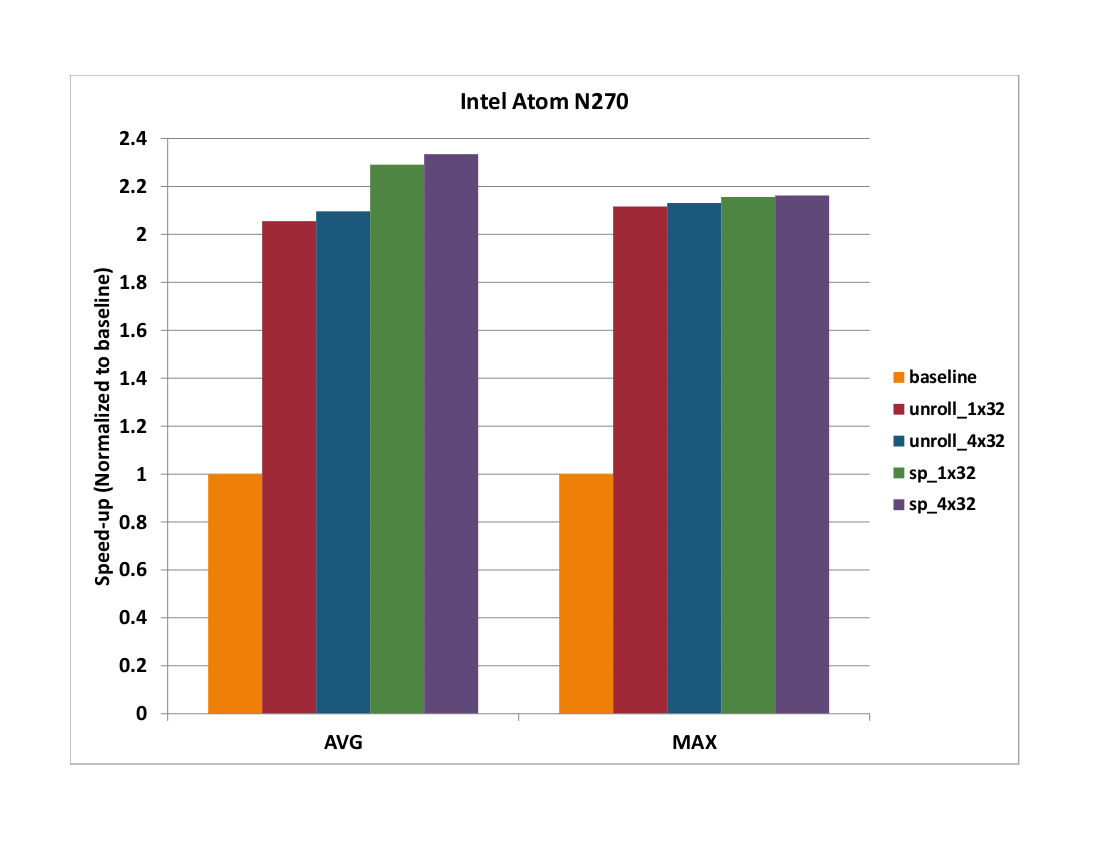
\includegraphics[scale=.5]{gemv_atom.png}
\end{center}
\caption{Relative speedup of GEMV on the Intel Atom.}
\label{fig:gemv_atom}
\end{figure}

\begin{figure}[ht]
\begin{center}
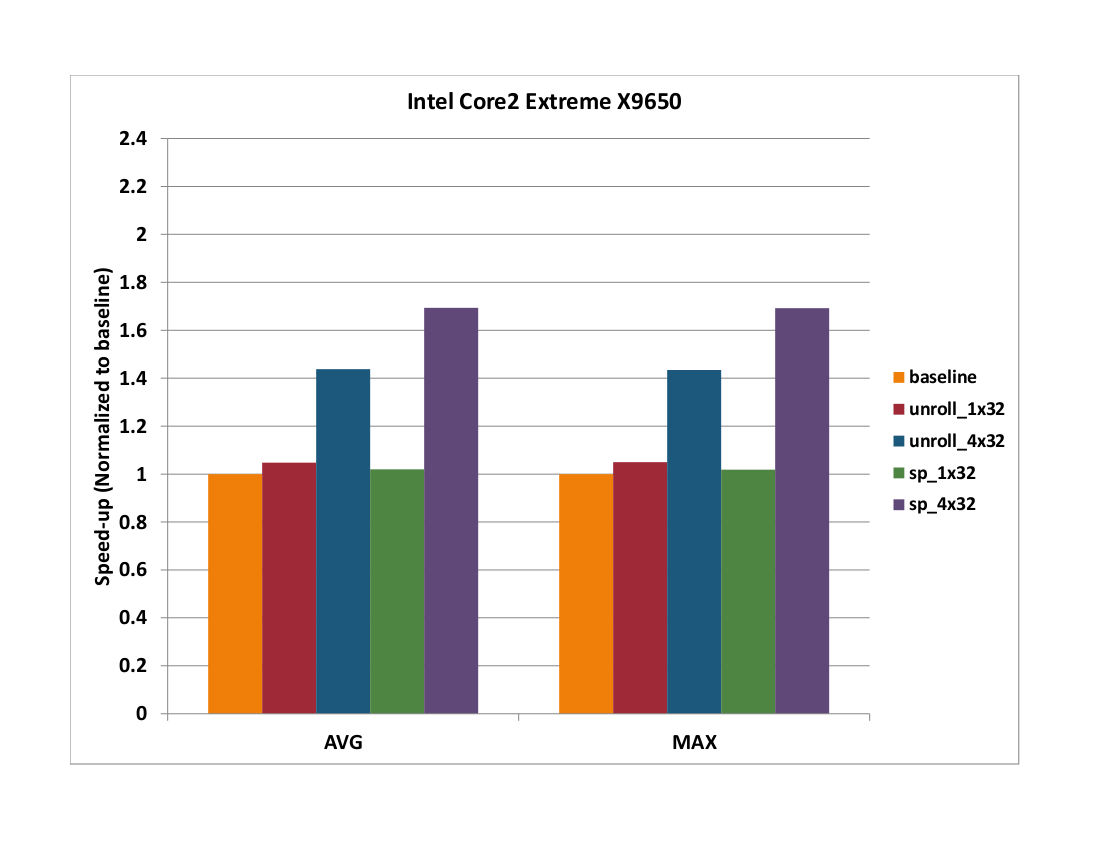
\includegraphics[scale=.5]{gemv_core2_extreme_x9650.png}
\end{center}
\caption{Relative speedup of GEMV on the Intel Core2 Extreme X9560.}
\label{fig:gemv_core2}
\end{figure}


\begin{figure}[ht]
\begin{center}
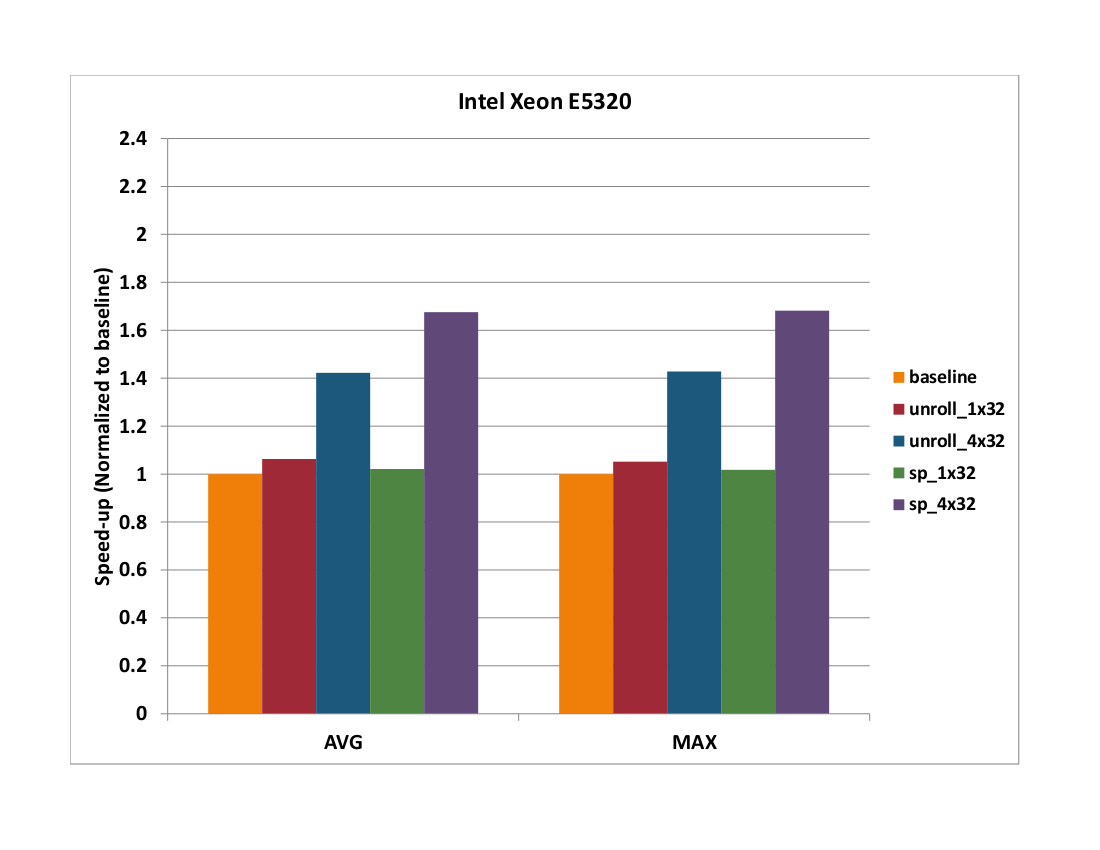
\includegraphics[scale=.5]{gemv_xeon_e5320.png}
\end{center}
\caption{Relative speedup of GEMV on the Intel Xeon E5320.}
\label{fig:gemv_corei7}
\end{figure}


\section{Surprises and Lessons Learned}
\begin{verbatim}
\end{verbatim}

\section{Conclusion}
\begin{verbatim}
+
+
+
+ Future work:
  - We have incorporated delays in our system, the question is can we use the
    results from hardware counters to determine the best values for these?
\end{verbatim}

\section{Post-mortem and Final Notes}

We propose distributing the credit as XX\% to Richard, XX\% to Flávio and XX\% to Berkin.
XXX Richard did this, Flavio did that, Berkin did ...

\bibliographystyle{plain}
\bibliography{draft}
\end{document}

